(\#3 in 4.2) Show that $\mathcal{B}_s$ is a basis for a topology on $\mathbb{R}^2$. Specifically, show
that $\mathcal{B}_s$ satisfies conditions (1) and (2) of Definition 4.2.1 on page 74 of the text. When
proving that condition (2) holds, you may support your argument with diagrams. However, you must be
sure that your diagrams cover all possible cases, are clearly drawn and accompanied by an
explanation.\\\\


\begin{solution}\renewcommand{\qedsymbol}{}\ \\
    Let $\mathcal{B}_s$ be as given in class and in the text. Consider any point $(x,y)\in\mathbb{R}^2$.
    Then take $S_{\epsilon}((x,y))$, the square centered at $(x,y)$, for any $\epsilon>0$. Then
    $(x,y)\in S_{\epsilon}((x,y))$. Since $(x,y)$ was arbitrary, we have that
    $\bigcup_{B\in\mathcal{B}_s}B=\mathbb{R}^2$ and $\mathcal{B}_s$ covers $\mathbb{R}^2$. Now, fix
    $(x_1,y_1), (x_2,y_2)\in\mathbb{R}^2$ and let
    $S_{\epsilon_1}((x_1,y_1)), S_{\epsilon_2}((x_2,y_2))\in\mathcal{B}_s$ be such that
    $S_{\epsilon_1}\cap S_{\epsilon_2}\neq\emptyset$, and let
    $(x,y)\in S_{\epsilon_1}\cap S_{\epsilon_2}$. Now take
    $\epsilon_3=min\{\epsilon_1-max\{|x-x_1|,|y-y_1|\}, \epsilon_2-max\{|x-x_2|, |y-y_2|\}\}$. Also take
    $(x_3,y_3)\in\mathbb{R}^2$ where
    
    $$x_3=\frac{max\{|x-x_1|<\epsilon_1, |x-x_2|<\epsilon_2\}
    +min\{|x-x_1|<\epsilon_1, |x-x_2|<\epsilon_2\}}{2}$$
    
    and
    
    $$y_3=\frac{max\{|y-y_1|<\epsilon_1, |y-y_2|<\epsilon_2\}
    +min\{|y-y_1|<\epsilon_1, |y-y_2|<\epsilon_2\}}{2}$$
    
    That is, we are setting $(x_3,y_3)$ to be the midpoint of the intersection of $S_1$ and $S_2$. Then
    $S_{\epsilon_3}((x_3,y_3))\in\mathcal{B}_s$ such that
    $(x,y)\in S_{\epsilon_3}((x_3,y_3))\subseteq S_{\epsilon_1}((x_1,y_1))\cap
    S_{\epsilon_2}((x_2,y_2))$
    as shown in the diagram below. Here we show squares to be in the first quadrent for simplicity, but
    since the centers of $S_1$ and $S_2$ are arbitrary, this need not be the case. So, by the diagram,
    we see that when the intersection of 2 squares is non empty, there exists a square with length
    $\frac{\epsilon}{2}$ that is a subset of the intersection that contains the arbitrary point $(x,y)$.
    Thus, we have that $B_s$ is a basis for some topology on $\mathbb{R}^2$.

    \begin{center}
    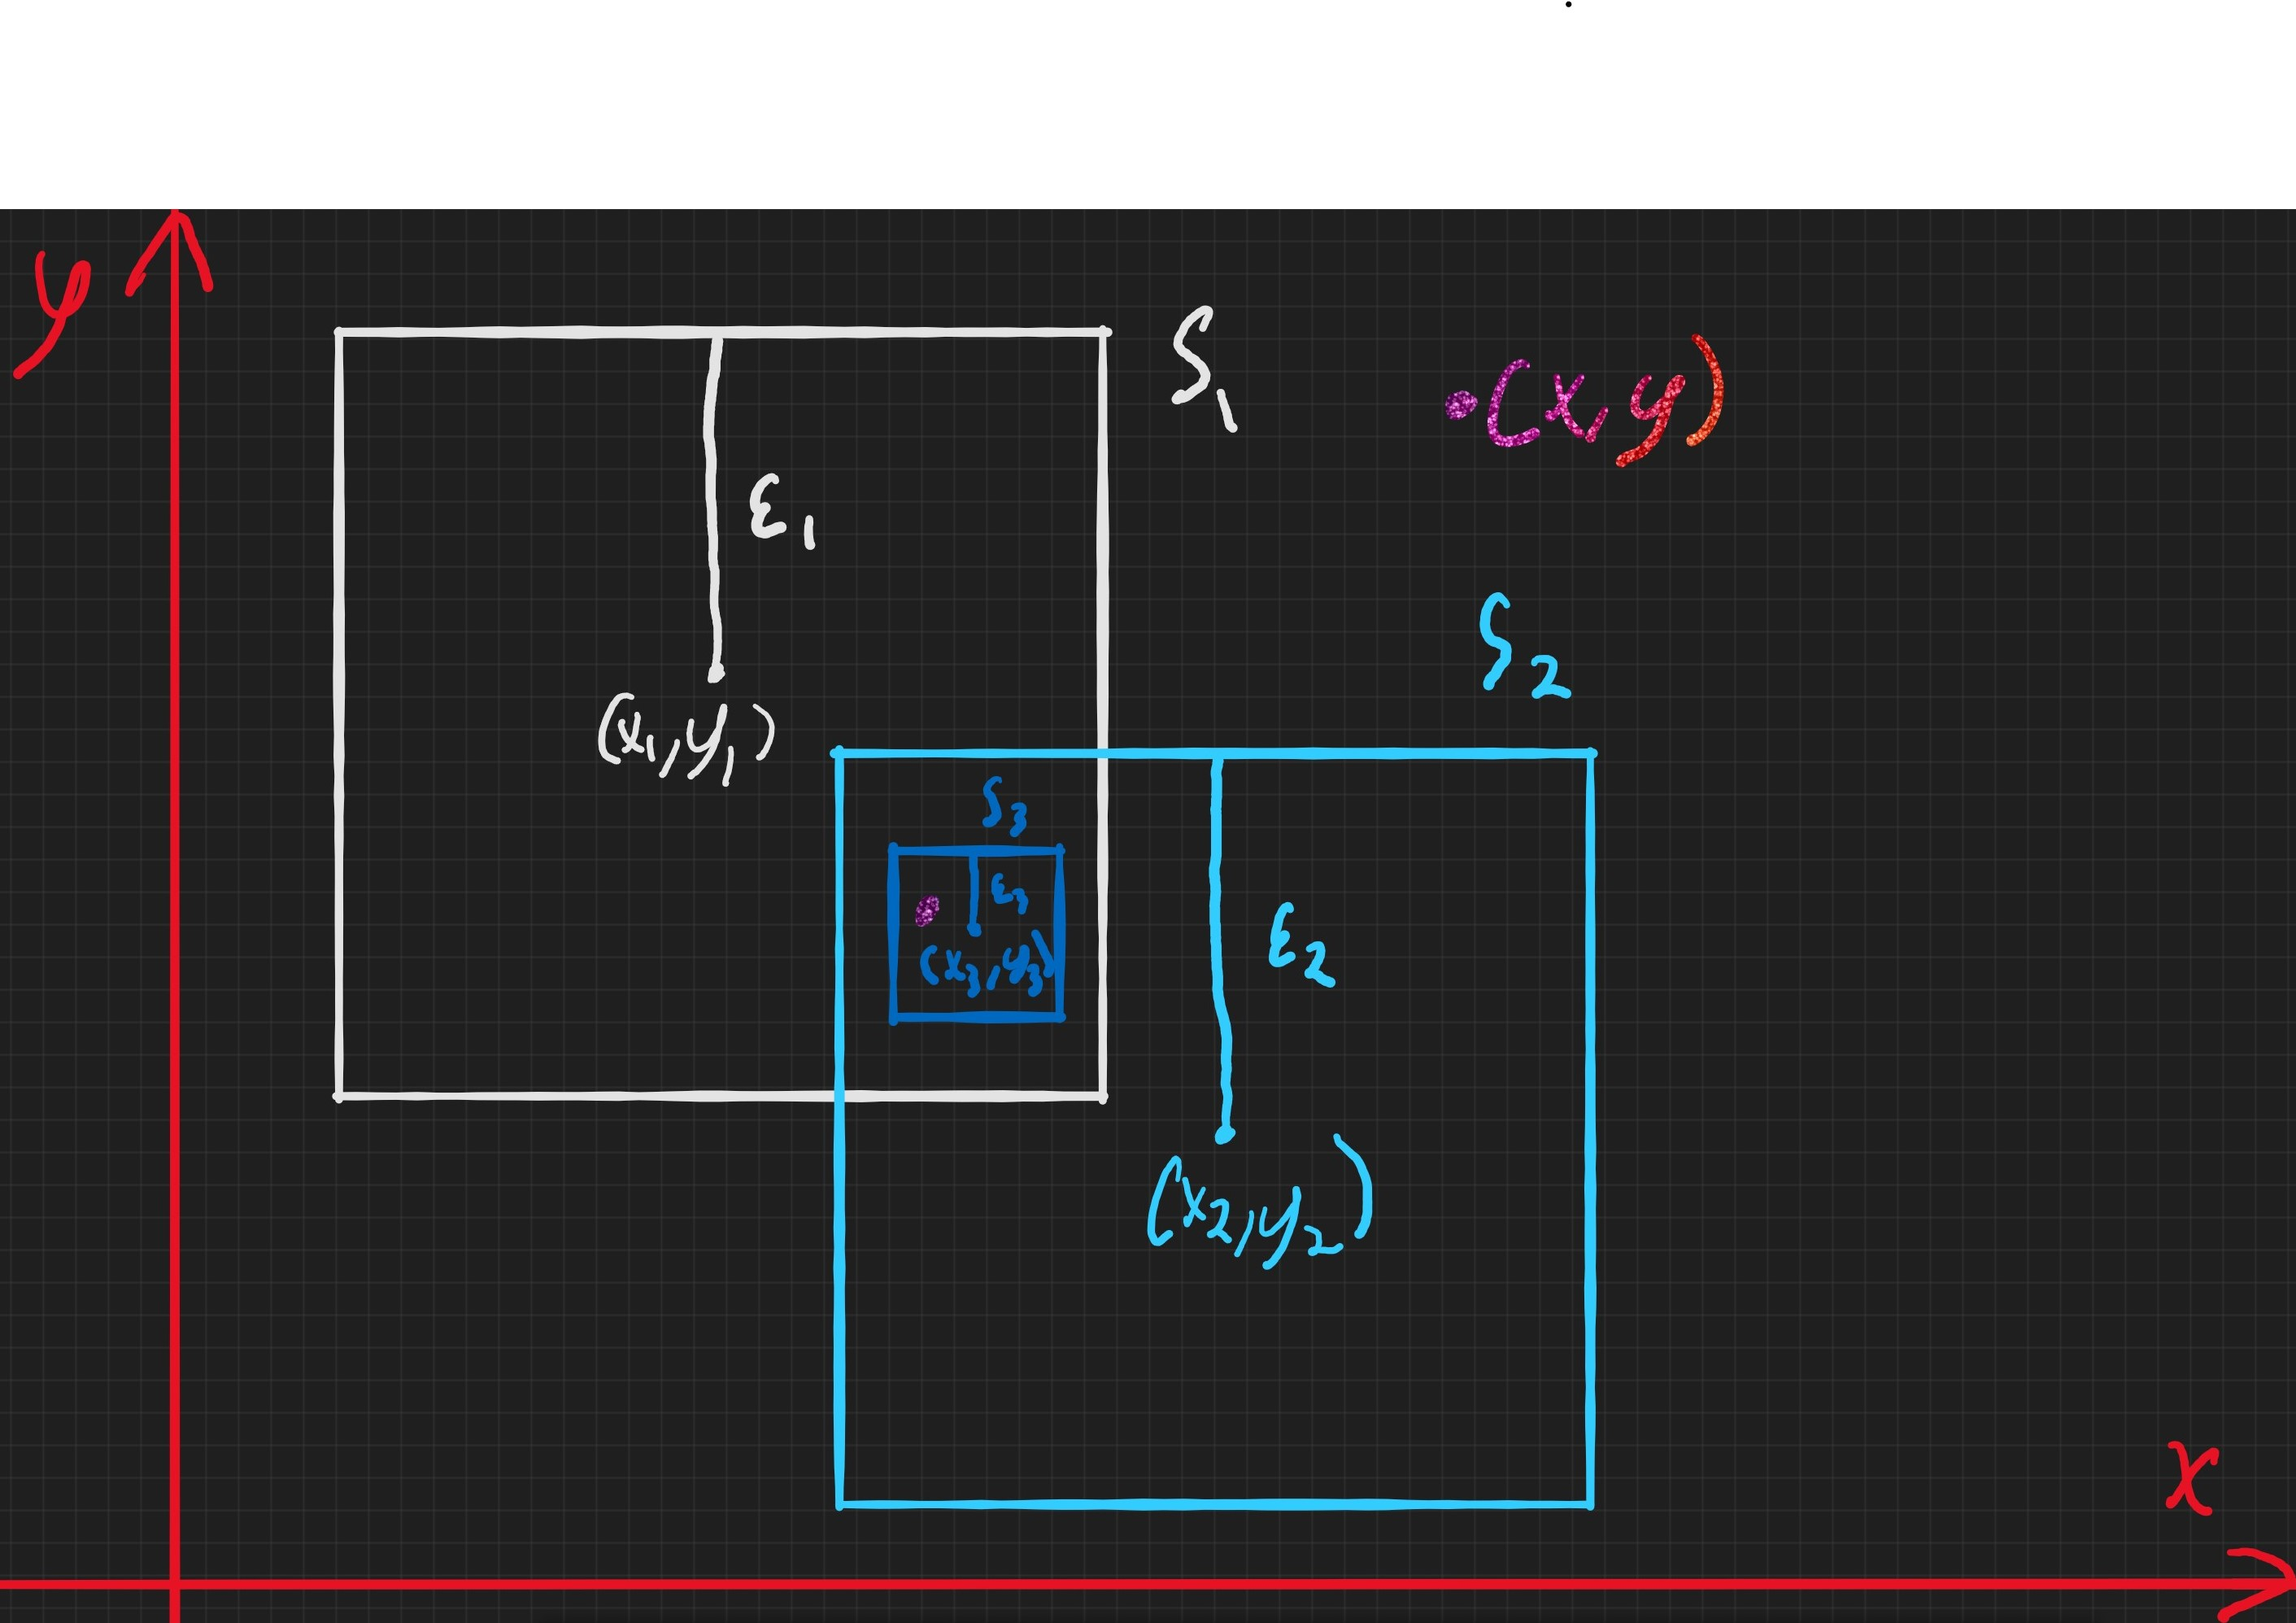
\includegraphics[scale=0.37]{ps5p1.JPG}
    \end{center}

\end{solution}